\documentclass[twoside,a4paper,12pt]{article}
\usepackage[applemac]{inputenc}
\usepackage{wrapfig}
\usepackage{graphicx}
\usepackage{graphics}
%\usepackage{subfig}
%\usepackage{inputenc}
\usepackage{amsmath}
\usepackage{amsfonts}
\usepackage{amssymb}
\usepackage[singlelinecheck=false]{caption}
\usepackage{array}
\usepackage{multirow}
\usepackage{setspace}
\usepackage{hyperref}
\usepackage{verbatim}
\usepackage[clearempty]{titlesec}
\usepackage{epstopdf}
\usepackage{lineno}
\usepackage{textcomp}
\usepackage{nicefrac}
\usepackage{xspace}
\usepackage{todonotes}
%\usepackage{autoref}
\usepackage[small, bf, hang, raggedright]{subfigure}

\usepackage[english]{babel} 

\onehalfspacing
\usepackage[left=2.9cm,right=2.9cm,top=3cm,bottom=4.5cm]{geometry}
\newcommand\leerseite{\newpage\thispagestyle{empty}\hspace{1cm}\newpage}

\newcommand{\subfigureautorefname}{\figurename}

\newcommand\piminus{\(\mathrm{\pi^-}\)}
\newcommand\muminus{\(\mathrm{\mu^-}\)}
\newcommand\eminus{\(\mathrm{e^-}\)}
\newcommand\eplus{\(\mathrm{e^+}\)}
\newcommand\geant{\textsc{Geant\,4}\xspace}

\begin{document}\selectlanguage{english}




\section*{Answers to Jerry's comments from 27.03.2016}
Dear Jerry,

Thank you for your comments. I will try to clarify further. 
Please again find my answers between your quotes below:


\begin{quote}\texttt{1) The modeling of the impact of contamination on the resolution is
convincing, and I concur the impact is negligible relative to other
uncertainties.}\end{quote}
Thank you!

\begin{quote}\texttt{2) With respect to energy versus hit density apparently the AHCAL
segmentation makes any differences small.   At some point we should
investigate this further with perhaps additional weighting for the cell
sizes.  But this is sufficient for now.}\end{quote}
Just a comment: Further studies in a similar direction are currently underway by Coralie Neub\"user and Huong Lan Tran here at DESY. 

Coralie is studying and comparing different energy reconstruction schemes (standard, software compensation, SDHCAL-like) with AHCAL data and simulations of various cell sizes. The existing note CAN-049 is currently updated (might be in collaboration review already) and will be available soon.

Lan is working on the implementation of software compensation into PandoraPFA and the resulting improvements in jet energy resolution in the context of ILD HCAL cell size optimisation.

Both of these studies should result in insights on how energy reconstruction schemes behave for different HCAL cell sizes, hopefully hinting on how to ideally combine the different cell sizes in the AHCAL physics prototype.  

Additionally I would personally like to improve on the general software compensation scheme by incorporating not only hit energy density information but also spatial distribution of hits. For example, the software compensation used in the ATLAS FCAL (as far as I know) does not use hit energy densities at all, but relies solely on the radial distance of a hit to the shower axis, reaching similar energy resolution improvements as seen in this study. So there is room for future ideas, but certainly not in this note.

\begin{quote}\texttt{3) My question was vague for which I apologize.   Maybe this is better:
Does the TCMT change the relative improvement gained from SC?  That is,
including the TCMT one gets the improvement between Standard and SC shown
in Fig 17.  If this same plot is made without the TCMT is the same
relative improvement seen.   This speaks to the algorithm development.}\end{quote}

As the general influence of the TCMT is rather small, and especially since the SC treatment of the TCMT is very rudimental, I have no reason to suspect any difference in resolution improvement from not including the TCMT. I could get you the numbers if you would rather know exactly.

\begin{quote}\texttt{4) REQUEST: With respect to formula 3, the extra text helps make this
clearer.  Has the behavior been confirmed by cutting plot 10b on high EM
showers and high HCAL showers?}\end{quote}
If I understand correctly, what you are asking for is a confirmation for the claim that the software compensation scheme weights up hadronic-heavy showers and de-weights EM-heavy showers?
 
The only variable we have to judge whether a shower was particularly EM-heavy or hadronic-heavy is the ratio between standard and SC reconstructed energy as the ``mean SC weight'' of the event. Thus performing the cut you proposed would cut directly into the distribution shown in Fig10b, making the whole argument somehow circular.

What can be shown to be definitely true is that the software compensation scheme weights up showers that show too low standard reconstructed energy and weights down showers that show too high standard reconstructed energy, without knowledge of the true beam energy. The black markers shown in Fig 10.b indicate the mean (of y-values) of the distribution  in that x-axis bin. A black marker above the dashed grey diagonal thus indicates that the software compensation reconstruction (on average) reconstructs events in this range of standard reconstructed energy with a higher energy than the standard reconstruction. A black marker below the dashed grey diagonal indicates that the software compensation reconstructs events of this standard reconstructed energy with a lower energy than the standard reconstruction. As can be seen in Fig10.b, all black markers are above the diagonal for standard reconstructed energies below the beam energy of 32\,GeV and below the diagonal above the beam energy. 
This behaviour is seen for all beam energies. The textbook understanding of hadronic calorimetry accounts such behaviour to the varying EM fraction in hadron showers in combination with the non-compensating nature of most calorimeters.

I have attached the plots for standard reco energy vs. SC reco energy distributions for all beam data runs at the end of this document. I have added lines indicating the beam energy on both axes, do you think this helps to understand the message of the plot better? Then I would include this version into the draft as well. 

\begin{quote}\texttt{5) REQUEST:  I  still have difficulty understanding why the first two bins
in Fig 9 are slanted.  Could you perhaps explains in terms of Equation 3?
Are the weights for these two bins handled differently than the other two
bins?}\end{quote}

Ok. I will first motivate the counting of hits vs. always using the deposited energy, then I will explain what is actually done in my software and finally I will try to explain how the slanted bins 
shown in Fig.9 are exactly equivalent to that. So bear with me for a moment please:

In a sandwich-sampling calorimeters only a fraction of the total deposited energy is measured in the active layers. The actually deposited energy is reconstructed by multiplying the measured depositions in the active layers by the known sampling ratio. The spectrum of deposited energy of a MIP-like particle going through one of our scintillator cells resembles a slightly widened Landau-distribution with a long tail to high hit energies (see Fig 1.a of the draft). Due to the typically small sampling fractions of sampling calorimeters, multiplying the deposition of a single MIP that randomly fluctuated away from its 1\,MIP most probable value will propagate these Landau fluctuations into the full reconstructed energy, deteriorating the energy resolution. Instead of using the deposited energy of the particle, simply counting the number of particles and hits effectively reduces the effect of such Landau fluctuations on the reconstructed energy resolution.

For sake of simplicity, let's assume a slightly simplified SC energy reconstruction formula, only using the HCAL and disregarding the exclusion of the primary track from the SC weighting:
\begin{align}
  E_\text{rec}^\text{SC}=w_{\text{HCAL}} \cdot\left( \sum_{i}^{\text{bins}}\beta_i\left(E_\text{est.}\right)\cdot E^\text{HCAL}_i\right)
\end{align}

To generate the array $E_i^\text{HCAL}$ (as used in the formula above) for a given event first all entries are initialised to 0. For each hit I determine its corresponding hit energy bin $i_\text{hit}$ from its hit energy. For hits falling into bin no.3 and higher, the hit energy of the current hit is added to the array value at the index $i_\text{hit}$. So effectively I sum up the hit energies for each hit energy bin for bins 3--8. For hit energies falling into bin 1 and 2 I do not sum up the hit energies. Instead I just count the number of hits falling into these two bins separately. At the end of this procedure my array $E_i^\text{HCAL}$ holds the number of hits falling into hit energy bin 1 and 2 for $i=1..2$, while for $i=3..8$ it holds the sum of hit energies falling into these hit energy bins. This means bins 1--2 have a different unit (number of hits) than bins 3--8 (energy sum normalised to MIPs), but the needed conversion factor (it is known that the mean deposited energy of a MIP passing through one of our scintillator cells is around 1.4 MIP units) is automatically optimised in the optimisation.

The value of each bin in $E_i^\text{HCAL}$ is then weighted by the SC weighting parameter $\beta_i$. $\beta_i$ is parametrised by three parameters which are optimised by the $\chi^2$ method explained in the draft. The optimisation does not know or care whether bins in $E_i^\text{HCAL}$ are summing up hit energies or are only counting entries. So in the end the energy reconstruction formula given above is identical whether counting bins are used or not. The only difference is how the 8 entries of $E_i^\text{HCAL}$ are generated. Of course the parameters need to be reoptimised every time the definition of $E_i^\text{HCAL}$ entries changes.

If we introduce a hit energy dependent weight of the form $w(e) = \frac{a}{e}$, summing up over all hit energies weighted by this weight will yield the number of events:
\begin{align}
 \sum_i^N w(e_i)\times e_i 	&= \sum_i^N \frac{a}{e_i}\times e_i \\
				&= a \sum_i^N 1\\
				&= aN
\end{align}
$a$ is exactly the optimised value of $\beta_1$ and $\beta_2$ for a given $E_\text{est.}$.

So instead of explaining the different units used for weights in bins 1..2 and bins 3..8, applying the trick with energy dependent weights homogenises the representation of the weighting plot. The $\frac{a}{e}$ energy dependent weight exactly corresponds to the slopes in the bins shown in Fig.9(c,d). Also note that there is a second x-axis at the top of these plots showing the corresponding hit energy in MIPs.

This way of plotting weights of counting bins was introduced to be able to directly compare the optimised weights used in the SDHCAL analysis (which uses only three hit energy bins, all of which are counting entries) to software compensation weights, as will be shown in the upcoming update of CAN-049 (and has been shown at CALICE meetings before).

This seems really hard to explain well in written text. I am not sure if this is any clearer than before. If you have further questions please ask. 

\begin{quote}\texttt{6) V1-2 Plot 17 nicely shows that the weight discrepancies between MC and
Data do not have a strong impact and adequately addresses my question
about 25 and 50\% changes of the weights in the first and last bins.}\end{quote}
OK, thank you.

\begin{quote}\texttt{7) Since 12 GeV has the worst linearity for both standard and SC
reconstruction, this impact on this analysis is not so important.  Maybe
we would learn more with additional beam energies, Yes, I would suggest
including the fits for all the data should be in an appendix as a matter
of record.  Maybe just collected on a single page.}\end{quote}
For reasons unknown to me, there were no pion runs taken between 4\,GeV and 12\,GeV with the combined ScECAL+AHCAL setup at FNAL2009. Adding more beam energies and extending the beam energy range would also help to answer the question whether the parametrisation of the SC weights as 2nd order polynomials is truly adequate. Some of that will be answered in Coralie's upcoming update of CAN-049, as she is using the same software compensation scheme with very similar parametrisations on a wider energy range. 

Cheers,
Oskar

\clearpage
\begin{figure}[htbp]
\begin{center}
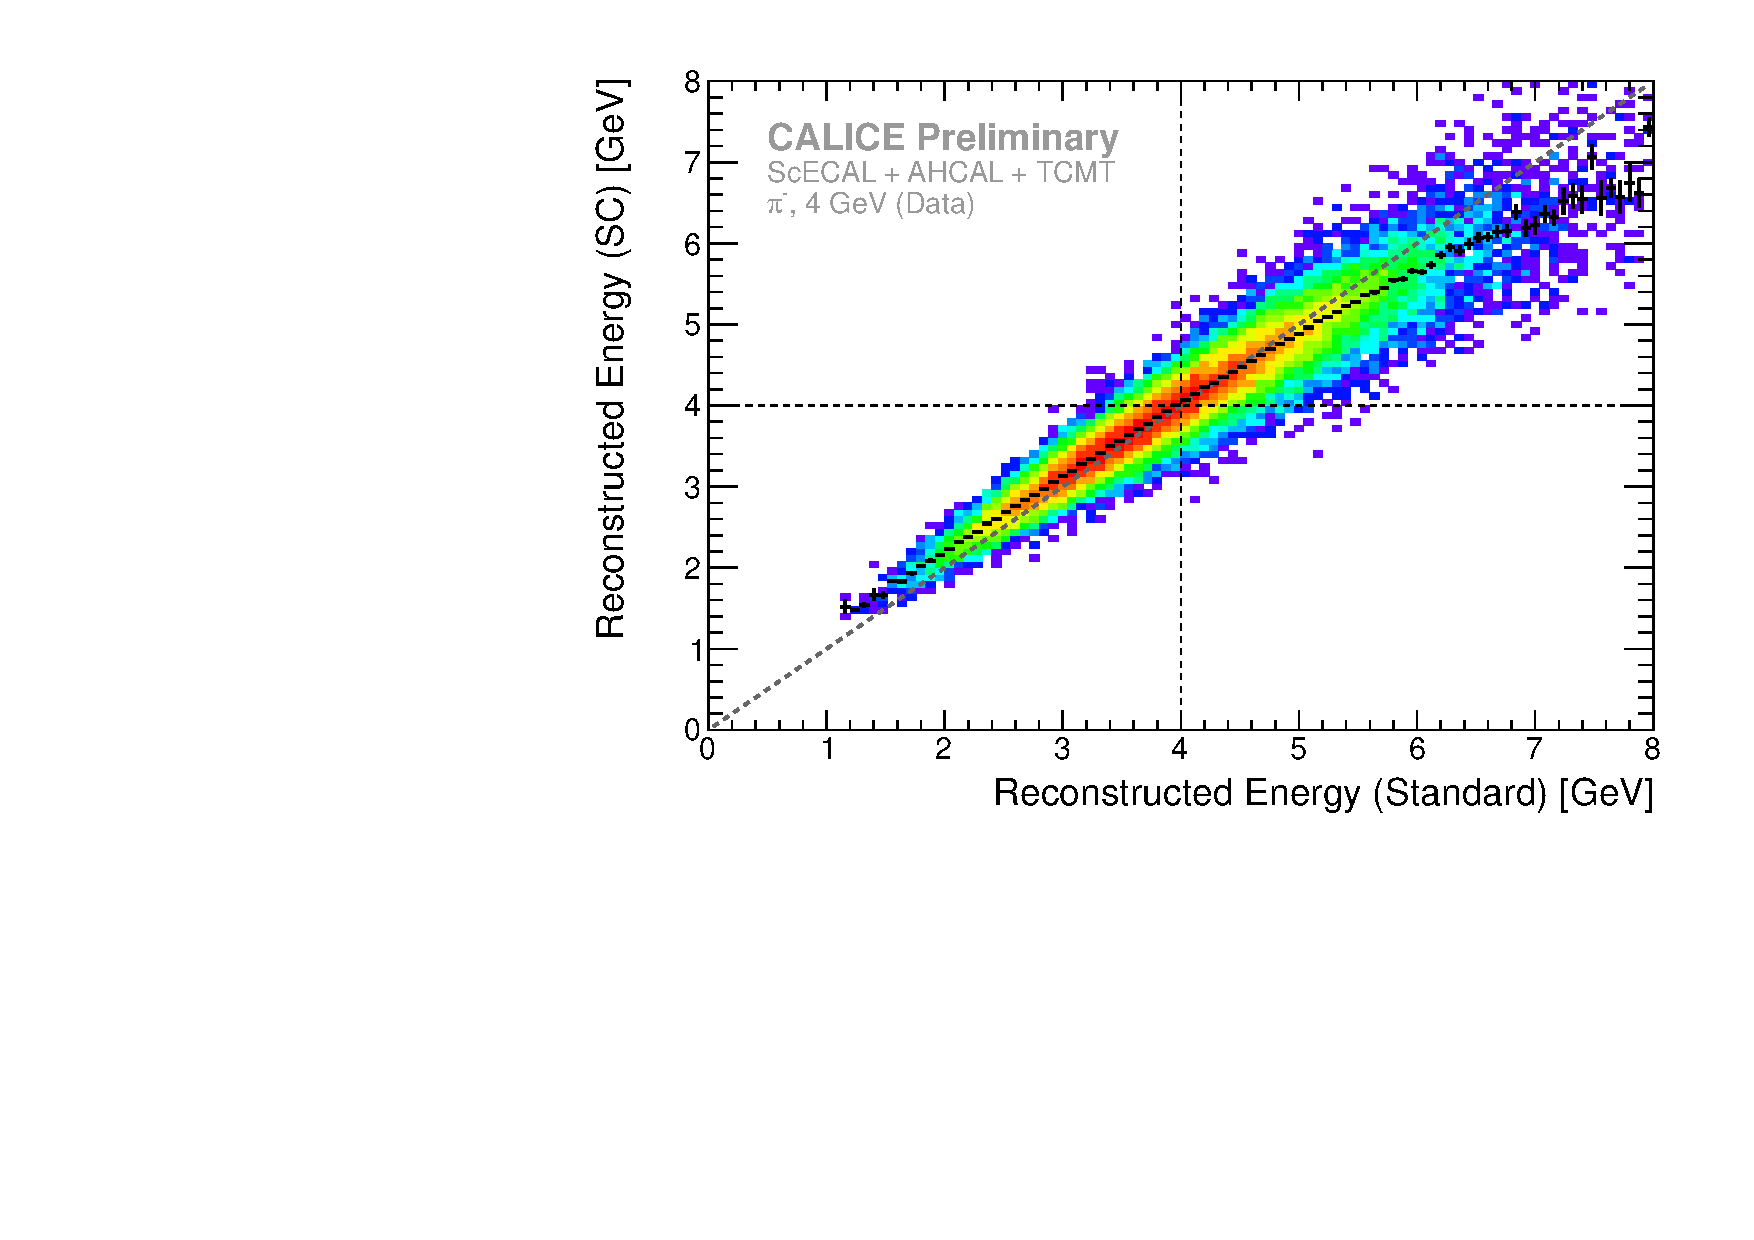
\includegraphics[width=1\textwidth,page=1]{ERec_corr_560506_data}
\caption{Correlation standard vs. software compensation reconstructed energy. 4\,GeV \piminus.}
\label{fig:erec_4gev}
\end{center}
\end{figure}

\begin{figure}[htbp]
\begin{center}
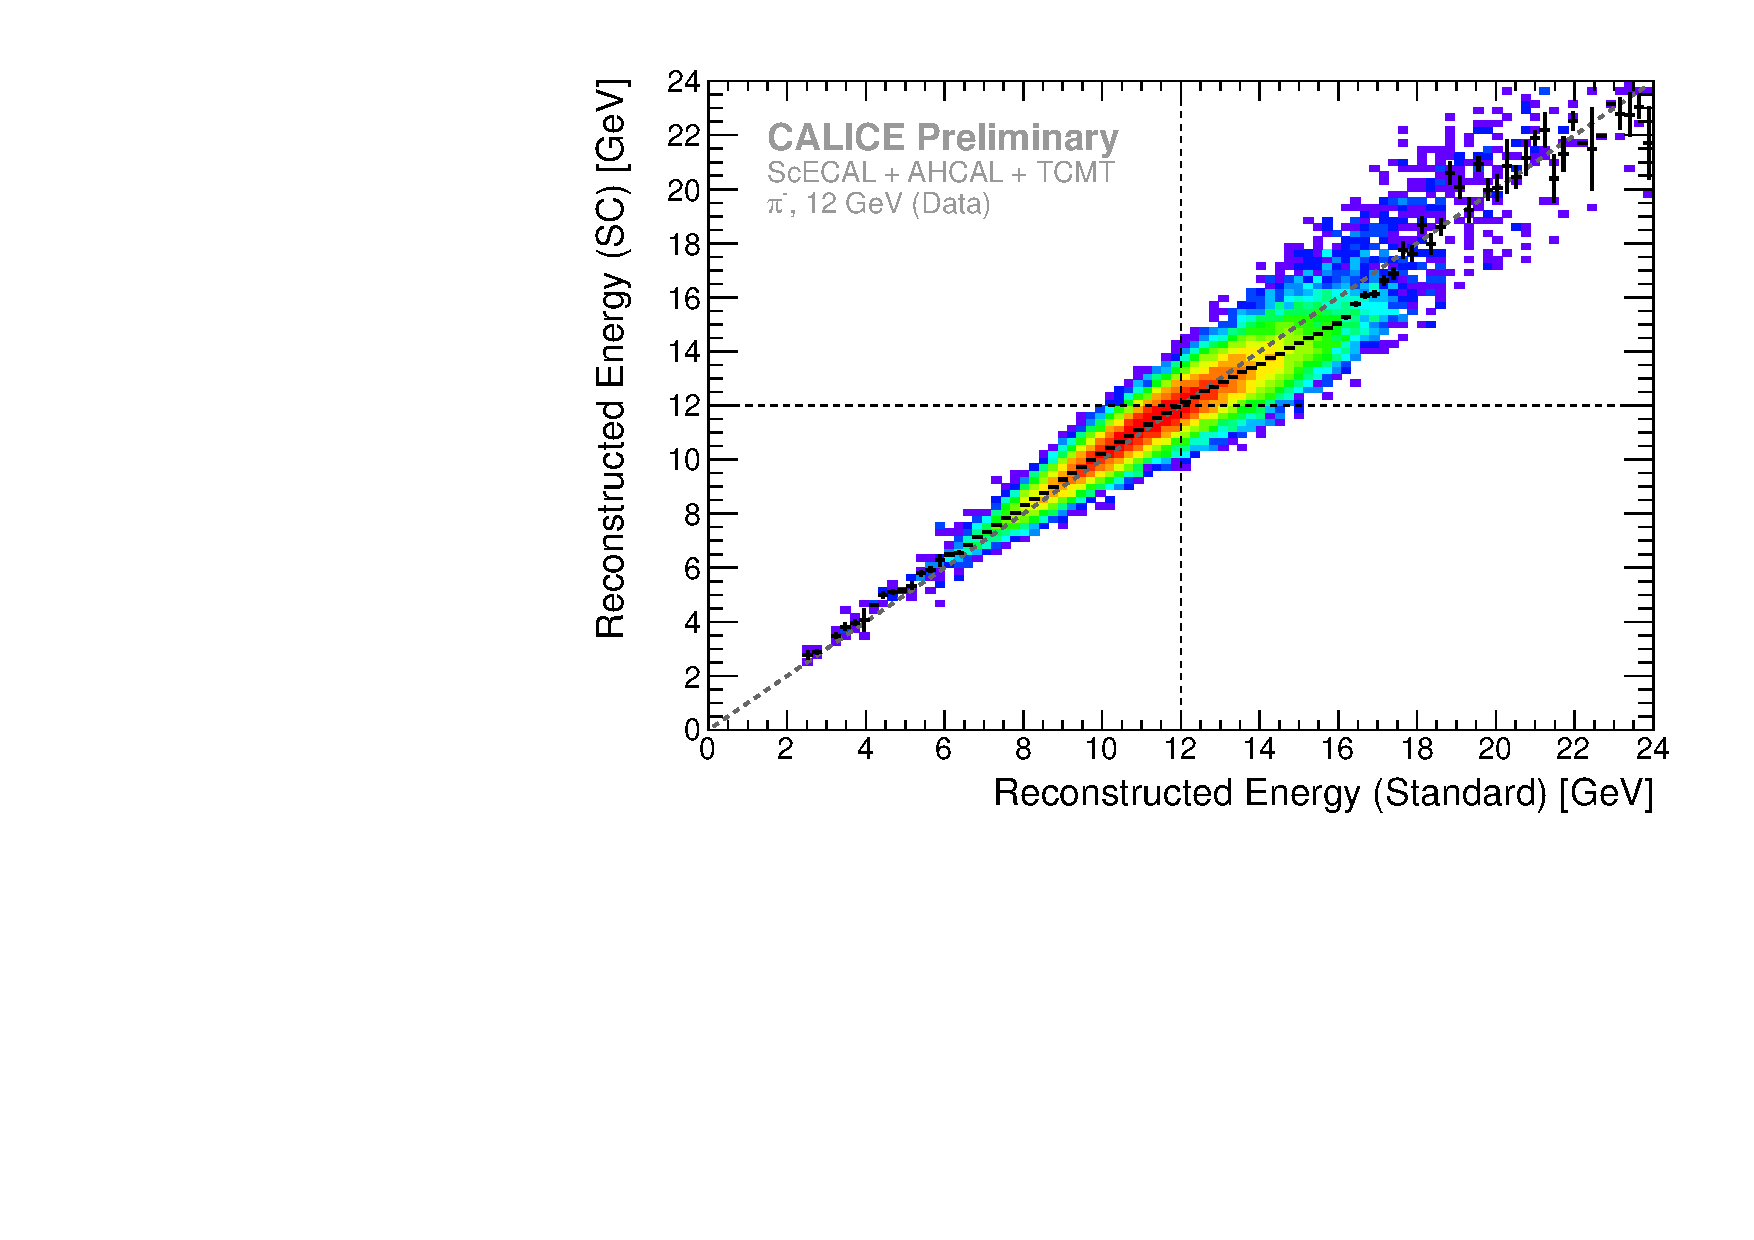
\includegraphics[width=1\textwidth,page=1]{ERec_corr_560498_data}
\caption{Correlation standard vs. software compensation reconstructed energy. 12\,GeV \piminus.}
\label{fig:erec_12gev}
\end{center}
\end{figure}

\begin{figure}[htbp]
\begin{center}
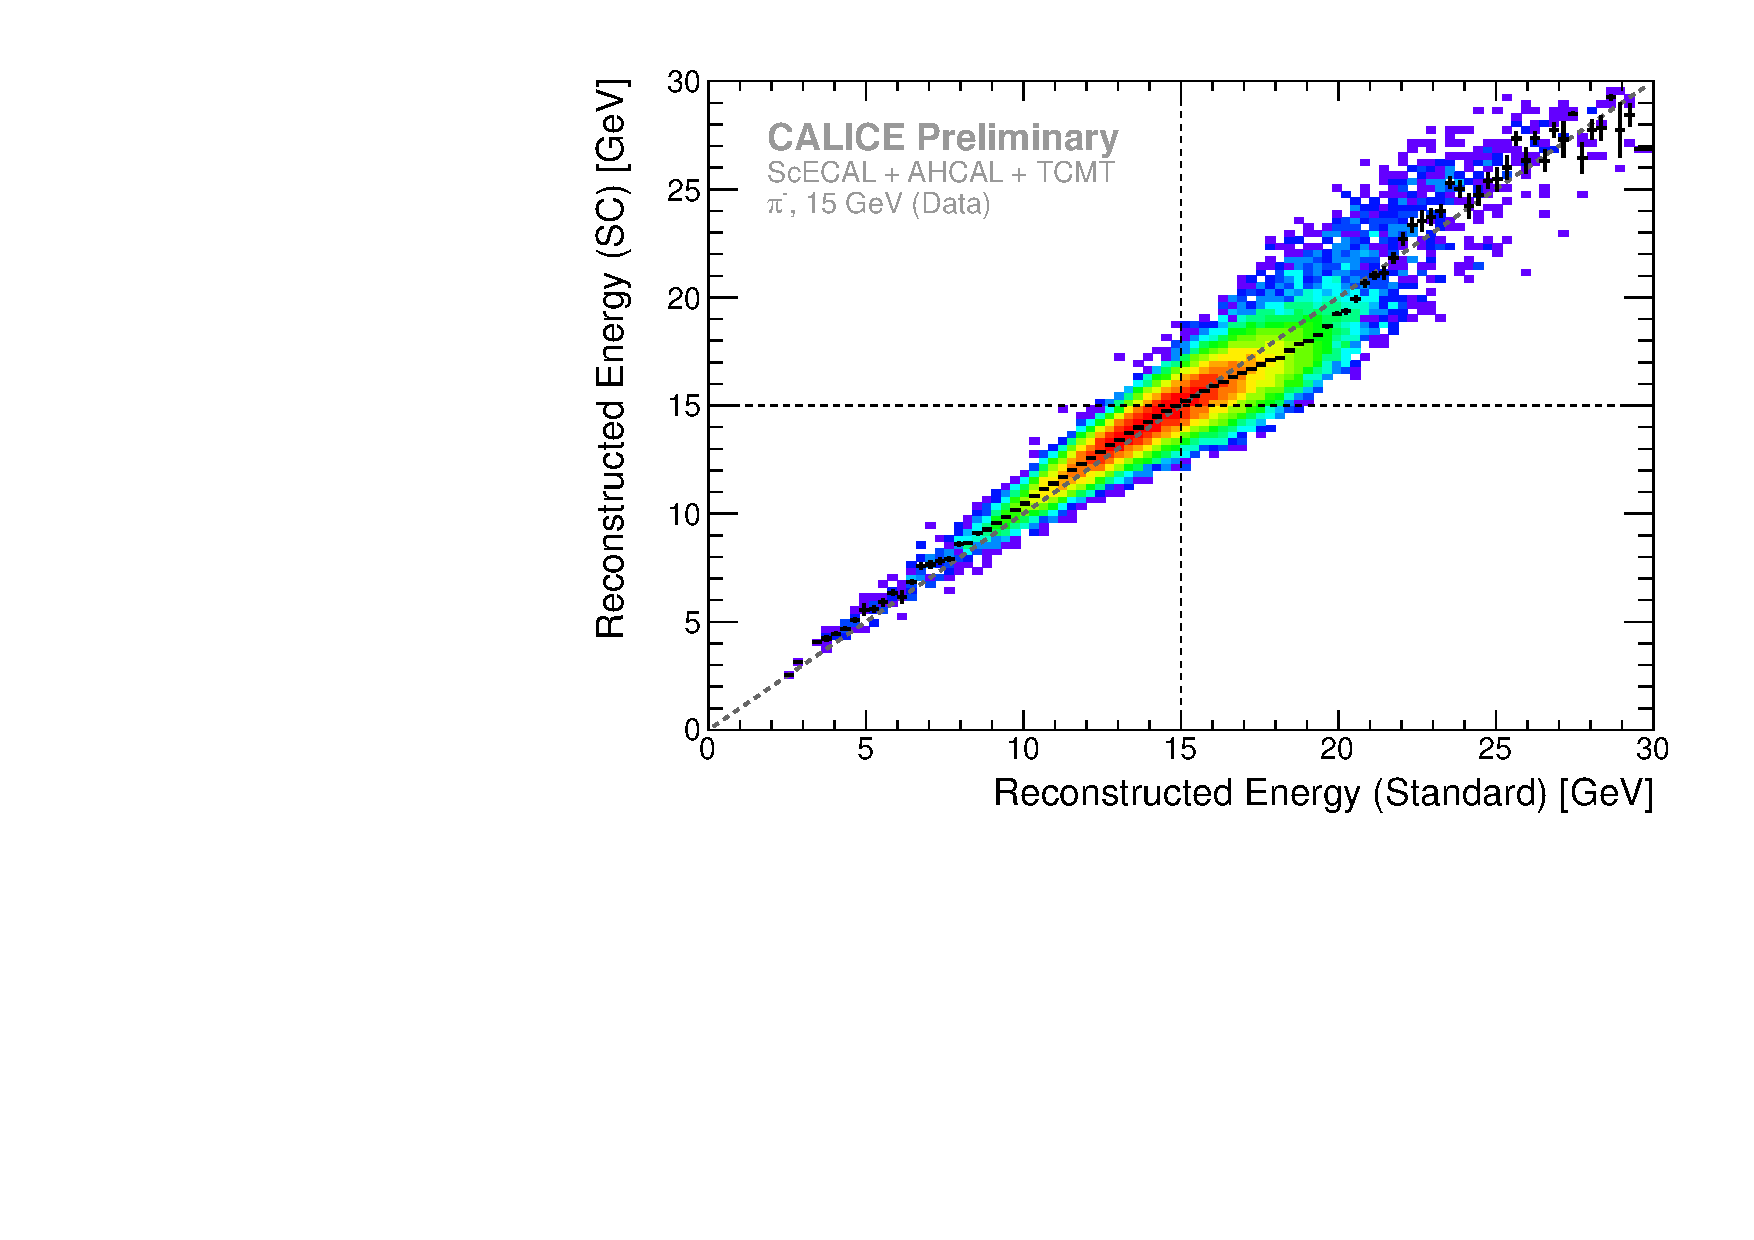
\includegraphics[width=1\textwidth,page=1]{ERec_corr_560496_data}
\caption{Correlation standard vs. software compensation reconstructed energy. 15\,GeV \piminus.}
\label{fig:erec_15gev}
\end{center}
\end{figure}

\begin{figure}[htbp]
\begin{center}
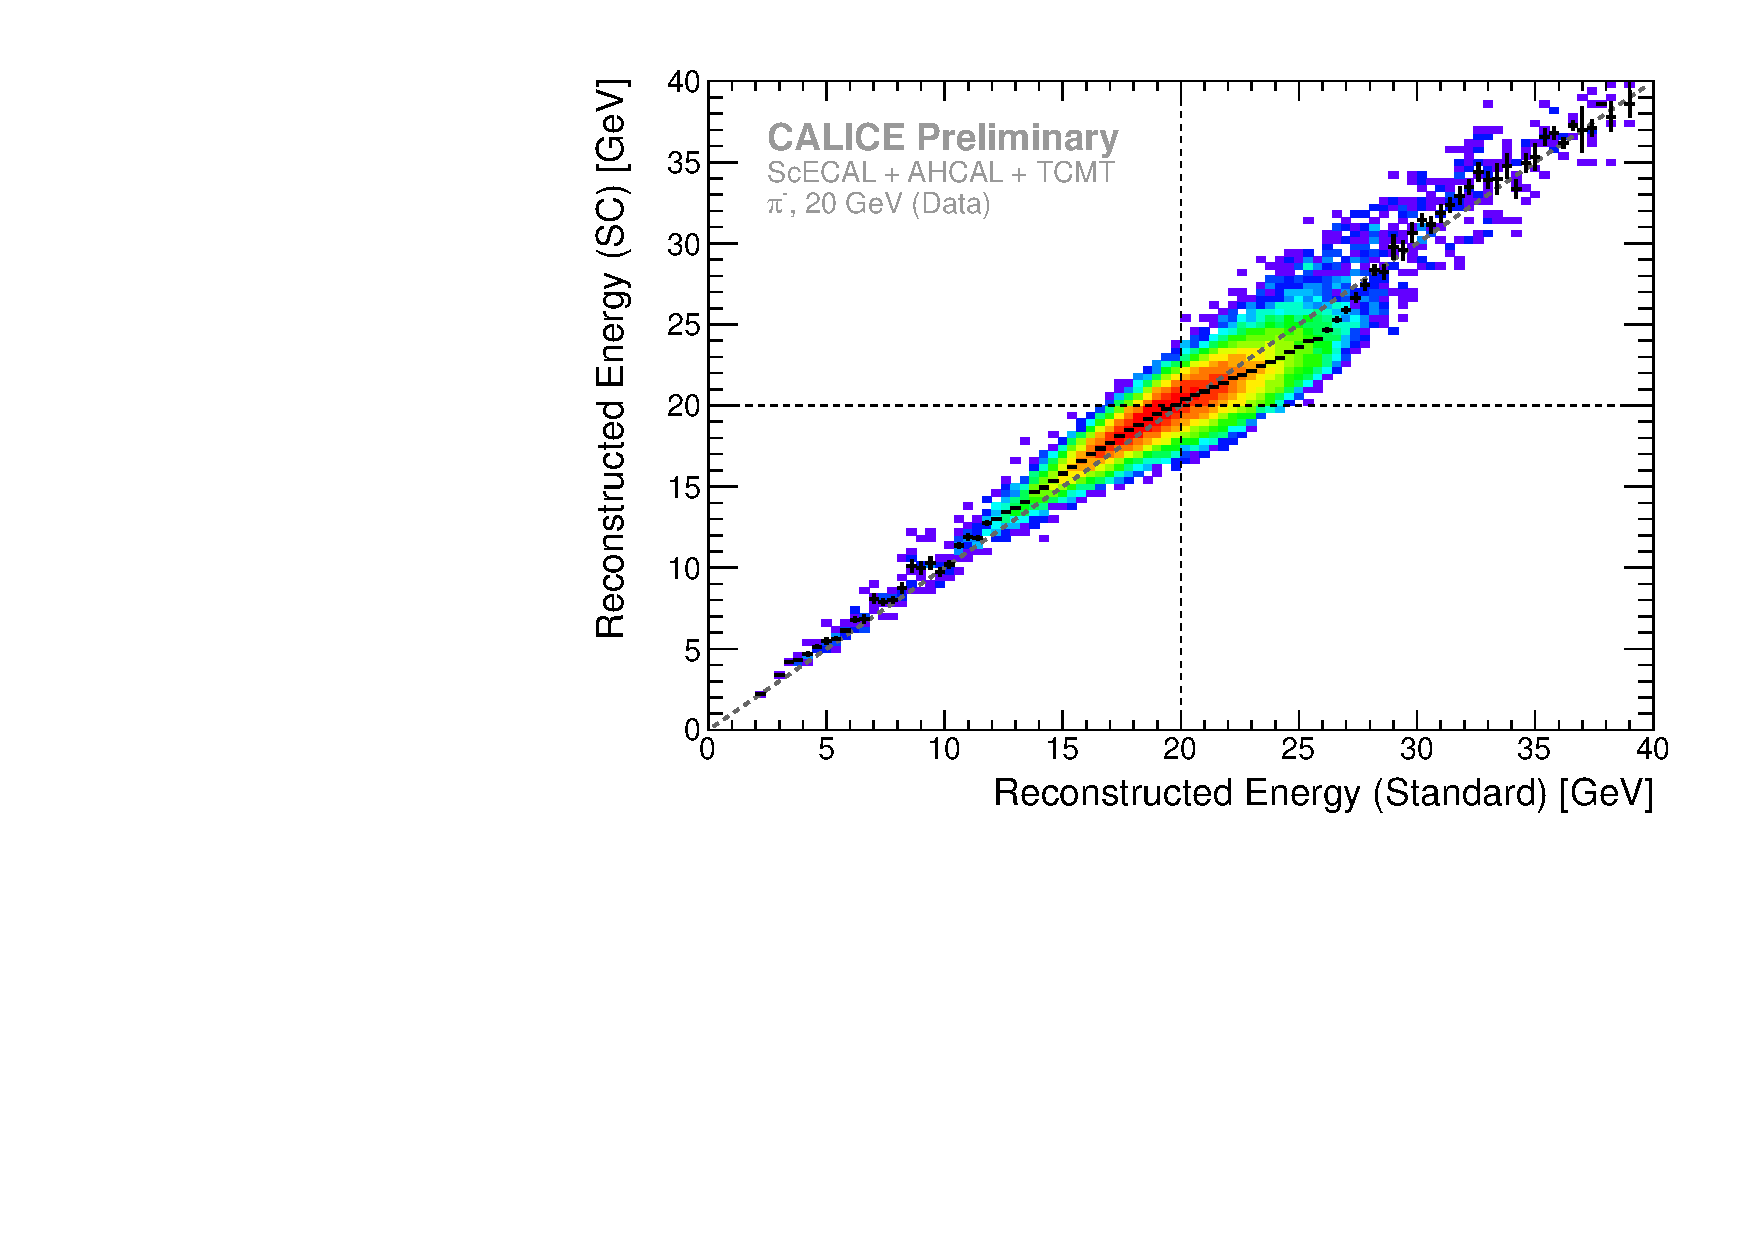
\includegraphics[width=1\textwidth,page=1]{ERec_corr_560481_data}
\caption{Correlation standard vs. software compensation reconstructed energy. 20\,GeV \piminus.}
\label{fig:erec_20gev}
\end{center}
\end{figure}

\begin{figure}[htbp]
\begin{center}
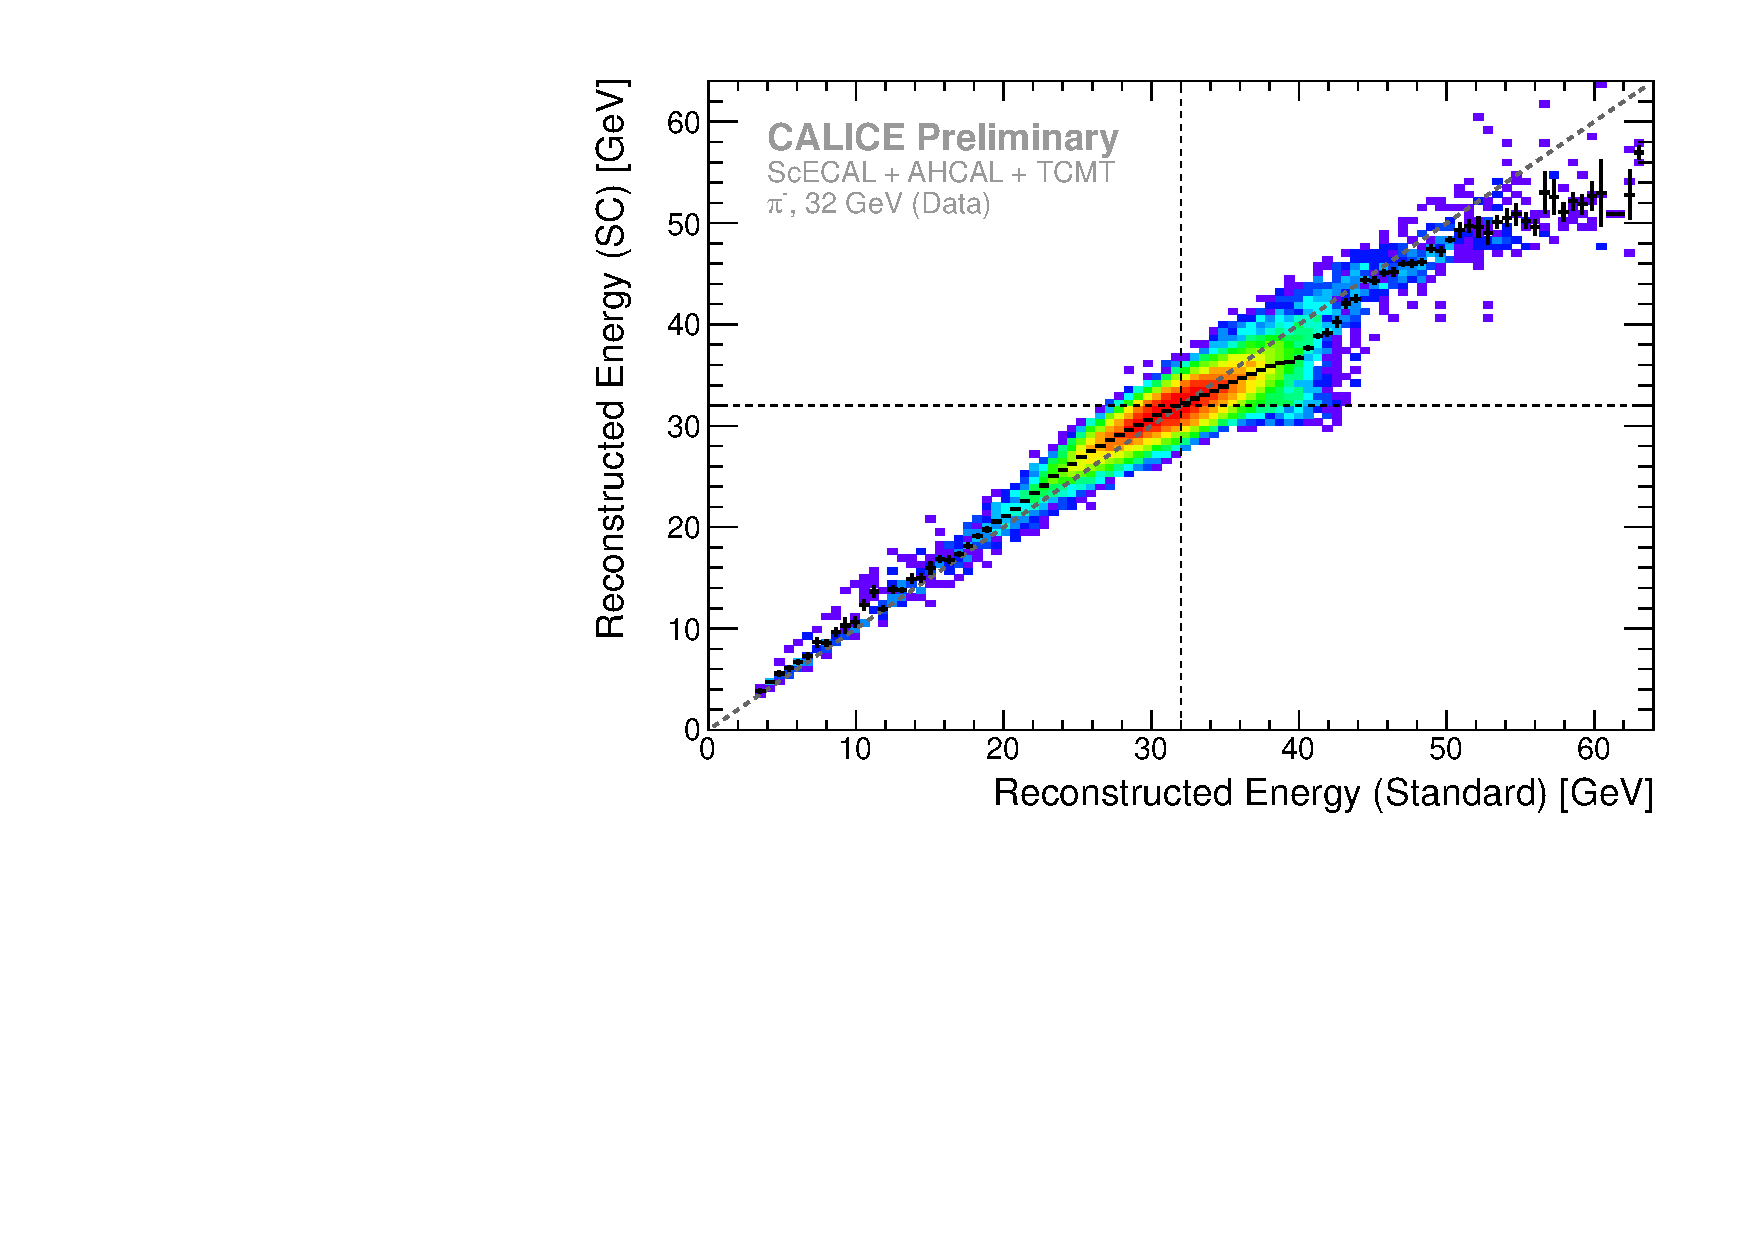
\includegraphics[width=1\textwidth,page=1]{ERec_corr_560474_data}
\caption{Correlation standard vs. software compensation reconstructed energy. 32\,GeV \piminus.}
\label{fig:erec_32gev}
\end{center}
\end{figure}


\end{document}
